\documentclass[12pt,DIV14,BCOR10mm,a4paper,twoside,parskip=half-,headsepline,headinclude,english,ngerman,bibliography=totocnumbered]{scrreprt}

\usepackage{hshhelper_base}

%%%%%%%%%%%%%%%%%%%%%%%%%%%%%%%%%%%%%%%%%%%%%%%%%%%%%%%%%%%%%%%%%%%%%%%%%%
\begin{document}    % hier gehts los
  \thispagestyle{empty} % Titelseite

\includegraphics[width=0.2\textwidth]{Wortmarke_WI_schwarz}

   {  ~ \sffamily
  \vfill
  {\Huge\bfseries Bedrohungsanalyse}
  \bigskip

  {\Large
  Dennis Grabowski, Julius Zint, Philip Matesanz, Torben Voltmer \\[2ex]
  Masterprojekt \enquote{Entwicklung und Analyse einer sicheren Web-Anwendung} \\
  Wintersemester 18/19
 \\[5ex]
   \today }
}
 \vfill

  ~ \hfill
  
\includegraphics[height=0.3\paperheight]{H_WI_Pantone1665}

\vspace*{-3cm}

\tableofcontents  % Inhaltsverzeichnis

\printbibliography

\chapter{Zur Analyse verwendeten Methoden}
\section{Dataflow Diagram}

\begin{figure}[htbp]
  \hspace*{-1.75cm}
  \label{overview-dfd-pic}
  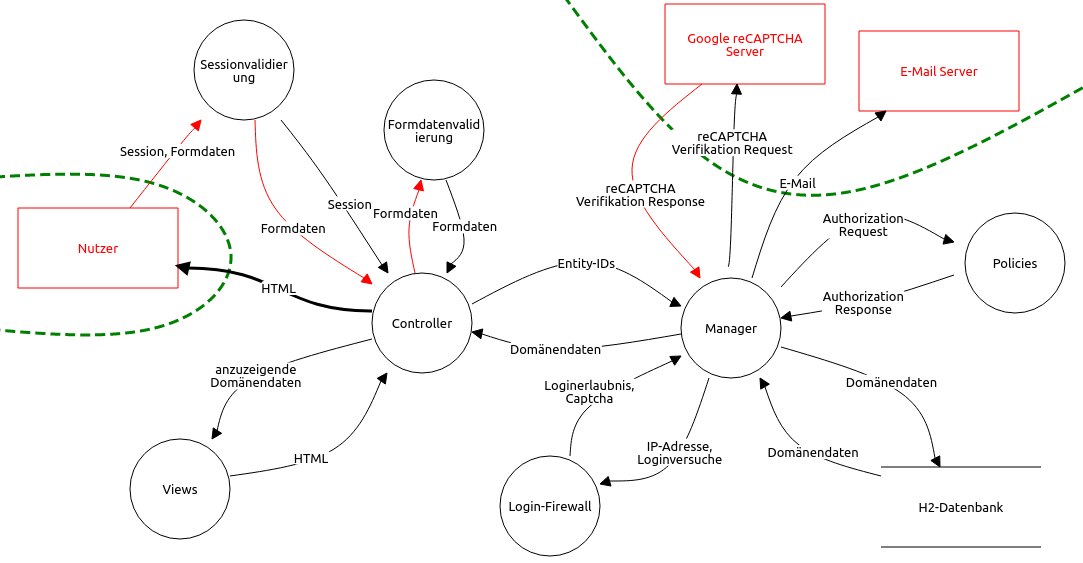
\includegraphics[width=1.25\linewidth]{resources/overview-dfd.jpg}
  \caption{Gesamtuebersicht des Datenflusses in unserer Applikation}
\end{figure}

\section{STRIDE}
\chapter{Bedrohungen}
\section{Gefundene Bedrohungen}

\subsection{Globale Bedrohungen}

\begin{itemize}
  \item \textbf{Spoofing des Servers}
  \begin{itemize}
  \item Zweck: Damit der Nutzer einem die Daten darlegt
  \item Möglichkeiten:
  \item Risiko: Mittelmäßig
  \item Gegenmaßnahmen: Authentication des Servers via Certificate (HTTPS/TLS), HSTS
  \end{itemize}

  \item \textbf{Eavesdropping}
  \begin{itemize}
  \item Zweck:
  \item Möglichkeiten:
  \item Risiko: Mittelmäßig
  \item Gegenmaßnahmen: HTTPS + HSTS oder SecureCookie
  \end{itemize}

  \item \textbf{Replayattacken}
  \begin{itemize}
  \item Zweck:
  \item Möglichkeiten:
  \item Risiko: Mittelmäßig
  \item Gegenmaßnahmen: HTTPS / CSRF
  \end{itemize}

  \item \textbf{Tampering}
  \begin{itemize}
  \item Zweck:
  \item Möglichkeiten:
  \item Risiko: Mittelmäßig
  \item Gegenmaßnahmen: HTTPS/TLS
  \end{itemize}

  \item \textbf{Ungueltig ausgestelltes Zertifikat (Tuerkischer Geheimdienst)}
  \begin{itemize}
  \item Zweck:
  \item Möglichkeiten:
  \item Risiko: Gering
  \item Gegenmaßnahmen: Cert Pinning
  \end{itemize}

  \item \textbf{DDOS (Out of scope)}
  \begin{itemize}
  \item Zweck: standard Zweck
  \item Möglichkeiten: standard means
  \item Risiko:
  \item Gegenmaßnahmen: None, or standard IDS
  \end{itemize}

  \item \textbf{XSS}
  \begin{itemize}
  \item Zweck:
  \item Möglichkeiten:
  \begin{itemize}
          \item Skript einbetten in Benutzername bei der Erstellung eines Nutzers
      \end{itemize}
  \item Risiko: Hoch
  \item Gegenmaßnahmen: CSP + alte Browser aussperren + Ausgabecodierung
  \end{itemize}
      Eingabevalidierung (Kleinbuchstaben und Zahlen, valide E-Mail-Adressen)

  \item \textbf{SQL Injection}
  \begin{itemize}
  \item Zweck:
  \item Möglichkeiten:
  \item Risiko: Hoch
  \item Gegenmaßnahmen:
  \begin{itemize}
    \item \texttt{ALLOW\_LITERALS=NONE}
    \item PreparedStatements
    \item Eingabevalidierung
  \end{itemize}
  \end{itemize}

  \item \textbf{CSRF}
  \begin{itemize}
  \item Zweck:
  \item Möglichkeiten:
  \begin{itemize}
          \item Einen fremden Benutzer ausloggen
          \item Einem Administrator einen Request unterjubeln, durch welchen er einen Nutzer erstellt
      \end{itemize}
  \item Risiko: Hoch
  \item Gegenmaßnahmen: CSRF-Tokens bei Requests checken
  \end{itemize}

  \item \textbf{Session faelschen (eine bestimmte oder irgendeine?)}
  \begin{itemize}
  \item Zweck: Client spoofen
  \item Möglichkeiten:
  \item Risiko: Hoch
  \item Gegenmaßnahmen: Signieren des Cookies durch PrivateKey und Verwendung von UUID, Bindung an IP-Adresse, Begrenzung der Lebenszeiten(?)
  \end{itemize}

  \item \textbf{Abstreitbarkeit illegaler Handlungen}
  \begin{itemize}
  \item Zweck:
  \item Möglichkeiten: Eintragen illegaler Namen bei Benutzernamen oder Gruppenmane
  \item Risiko: Gering
  \item Gegenmaßnahmen: Logging von IP + Zeit, Action, User
  \end{itemize}

  \item \textcolor{red}{Captcha loesen lassen von Indern?}
  \item \textcolor{red}{Elevation of privilege -> Frage an Peine. ?}
  \item \textcolor{red}{Security Header auflisten, warum welcher, wofuer}
\end{itemize}

\subsection{Domänenspezifische Bedrohungen}

\subsubsection{Moegliche Angriffe waehrend auf den Loginprozess}

\begin{itemize}
  \item \textbf{Ueberlanges PW beim Login eingeben}
  \begin{itemize}
  \item Zweck: Zum DDOSn der Applikation
  \item Möglichkeiten: Durch Eingabe eines ueberlangen Passworts braucht Hashing-Algo extra lange
  \item Risiko: Gering
  \item Gegenmaßnahmen: Constraint auf PW-Laenge
  \end{itemize}

  \item \textbf{Timing/Side-Channel auf Loginverhalten}
  \begin{itemize}
  \item Zweck: Herausfinden, ob Username existiert
  \item Möglichkeiten: Via abhoeren der Netzwerkverbindung, da Hashing/DB-Zugriff laenge des Requests beeinflussen
  \item Risiko: Mittelmäßig-Hoch
  \item Gegenmaßnahmen: Login Procedure fuer jeden Fall gleich ablaufen lassen
  \end{itemize}

  \item \textbf{Brute-forcing}
  \begin{itemize}
  \item Zweck: Zum Knacken eines Benutzeraccounts
  \item Möglichkeiten: Beispielsweise durch Wörterbuchattacken
  \item Risiko: Hoch
  \item Gegenmaßnahmen:
  \begin{itemize}
      \item Captcha Mode = Login nur moeglich, wenn Captcha geloest wird.
      \item Accounts muessen nach x falschen Logins, einen Captcha loesen, sowie IP-Adressen sperren nach Y falschen Logins
      \item Schwache Passwoerter verbieten
      \item Zwei-Factor-Auth
    \end{itemize}
  \end{itemize}
\end{itemize}

\subsubsection{Moegliche Angriffe beim Versand der Passwort-Reset-E-Mail}

\begin{itemize}
\item E-Mailversand abhoeren
  \begin{itemize}
  \item Zweck:
  \item Möglichkeiten:
  \item Risiko:
  \item Gegenmaßnahmen: SMTPS (Two-Faktor-Authentisierung)?
  \end{itemize}
\end{itemize}

\section{Ignorierte Bedrohungen}

\textcolor{red}{
Beispielsweise via Betriebssystem, physikalischer Zugriff auf der Maschine oder HTTPS?
Oder welche, fuer die es keine Motivation gibt, ggf. Repudiations
}

% Can be used to add a list of acronyms with their description
%\glsaddall
%\deftranslation{to=German}{Acronyms}{Abkürzungsverzeichnis}
%\deftranslation{to=German}{Glossary}{Glossar}
\printacronyms[title=Abkürzungsverzeichnis,toctitle=Abkürzungsverzeichnis]
\printglossary[type=main]

%\addcontentsline{toc}{chapter}{\listfigurename}
\listoffigures      % Abbildungsverzeichnis

%s\addcontentsline{toc}{chapter}{\listtablename}
% \listoftables       % Tabellenverzeichnis

\end{document}
